%%%%%%%%%%%%%%%%%%%%%%%%%%%%%%%%%%%%%%%%%%%%%%%%%%%%%%%%%%%%%%%%%%%%%%
%% Springer Nature LaTeX template (sn-jnl.cls v3.1)
%% Manuscript draft -- vehicle detection on UA-DETRAC
%%%%%%%%%%%%%%%%%%%%%%%%%%%%%%%%%%%%%%%%%%%%%%%%%%%%%%%%%%%%%%%%%%%%%%
%% Applied Intelligence (Springer) uses the numbered Springer Basic reference
%% style: citations in square brackets, references formatted as
%% "Author AB, Author CD (Year) Title. Journal Volume:Pages".
\documentclass[pdflatex,sn-basic,Numbered]{sn-jnl}% Applied Intelligence style

%%%% Standard Packages
\usepackage{graphicx}%
\graphicspath{{figures/}{./}}% resolve figures/ or same-directory layouts
\usepackage{adjustbox}% shrink over-wide tables to \textwidth (never enlarges)
\usepackage{multirow}%
\usepackage{amsmath,amssymb,amsfonts}%
\usepackage{amsthm}%
\usepackage[title]{appendix}%
\usepackage{xcolor}%
\usepackage{textcomp}%
\usepackage{manyfoot}%
\usepackage{booktabs}%
\usepackage{algorithm}%
\usepackage{algorithmicx}%
\usepackage{algpseudocode}%
\usepackage{listings}%
%%%% The class defines \bmhead as a level-5 (subparagraph) heading, so hyperref
%%%% reports "Difference (N) between bookmark levels". Loading bookmark after
%%%% hyperref (already loaded by sn-jnl.cls) rebuilds the PDF outline correctly
%%%% and removes those warnings without disabling bookmarks.
\usepackage{bookmark}%
%%%%

\raggedbottom

\begin{document}

\title[Parameter-Free Attention and a P2 Head for Small-Object Vehicle Detection]{Parameter-Free Attention and a High-Resolution Detection Head for Small-Object Vehicle Detection: A Multi-Seed and Cross-Initialization Study on UA-DETRAC}

%%=============================================================%%
%% Author information                                          %%
%% Z. Kang is the first author; X. Liu is the corresponding     %%
%% author and is therefore starred, following the sn-jnl        %%
%% template convention. Both share affiliation [1].             %%
%%=============================================================%%
\author[1]{\fnm{Zhitong} \sur{Kang}}\email{kangzt@stu2024.jnu.edu.cn}
\author*[1]{\fnm{Xiaoxiang} \sur{Liu}}\email{tlxx@jnu.edu.cn}

\affil*[1]{\orgdiv{School of Intelligent Systems Science and Engineering}, \orgname{Jinan University}, \orgaddress{\street{206 Qianshan Road, Xiangzhou District}, \city{Zhuhai}, \postcode{519070}, \state{Guangdong}, \country{China}}}

\abstract{Small-object detection dominates the error budget in traffic-surveillance imagery, and lightweight detectors are often modified with attention modules, extra prediction heads and refined regression losses. Such modifications are typically reported from a single run, evaluated on the split used to select the best checkpoint. This paper re-examines that practice on the UA-DETRAC vehicle-detection benchmark. We combine three lightweight modifications --- SimAM, a parameter-free energy-based attention module placed after each detection-head feature map, an additional P2 prediction level, and the EIoU regression loss --- and train all six ablation variants with three seeds, both from scratch (100 epochs) and from COCO-pretrained weights (25 epochs), scoring every model on the full validation set under two metric conventions. Overall mAP differences are small and never statistically significant across the configurations tested (largest gain $+0.0114$ mAP@[0.5:0.95], Welch $t$-test $p>0.05$). The P2 head is the only modification consistently at or near the top across settings, whereas EIoU never yields a positive overall effect and is significantly negative in two scene-level comparisons. Pretrained initialization raises the baseline by $+0.0062$ mAP@0.5 and absorbs most of the gain of the modifications. We argue that multi-seed, cross-initialization and two-protocol reporting should be the default for such claims.}

\keywords{object detection, small-object detection, attention mechanism, YOLOv8, UA-DETRAC, statistical significance}

\maketitle

\section{Introduction}\label{sec:intro}

Real-time vehicle detection from fixed traffic cameras underpins traffic monitoring, violation detection, and autonomous-driving perception. In such imagery the objects of interest are frequently small: a car observed from a gantry-mounted camera at tens of metres occupies only a few tens of pixels on the long side. Small objects are consequently the dominant contributor to detection error --- a difficulty that has been documented since the early evaluation studies of detection benchmarks \cite{dollar2012pedestrian} --- which is why the small-object regime receives disproportionate attention in the literature \cite{lin2017focal,cheng2023smallobject,kisantal2019augmentation,akyon2022sahi}.

A common recipe for improving small-object accuracy with a lightweight detector is to combine three ingredients: (i) an attention module that re-weights features, (ii) an additional high-resolution prediction level so that small objects are matched at a finer stride, and (iii) a refined bounding-box regression loss. For the widely used YOLOv8n model \cite{jocher2023ultralytics}, many published variants differ from the baseline only by such changes. The reported gains are typically in the range of a few tenths of a point to two points of mAP, and they are usually obtained from a single training run and reported on the same validation split that was used to select the best checkpoint.

This practice has two well-known weaknesses. First, a single run cannot distinguish a systematic improvement from seed noise; differences of this magnitude are frequently within run-to-run variation \cite{beyer2020imagenet,dietterich1998tests,demsar2006statistical}. Second, selecting the best checkpoint on the validation set and then reporting validation metrics is optimistically biased. Both effects are aggravated when the baseline is initialized from COCO-pretrained weights, because a strong initialization can absorb most of the benefit that a lightweight architectural change would otherwise provide.

This paper reports a study designed to expose and quantify these effects rather than to advertise a new state of the art. Our contributions are as follows.

\begin{enumerate}
\item We construct YOLOv8n-ASP, which combines SimAM \cite{yang2021simam} --- a parameter-free, energy-based attention module --- with an additional P2 prediction level and the EIoU regression loss \cite{zhang2022eiou}, and we implement it so that the attention module enters the network as a standalone, channel-preserving layer, requiring no modification of the model-parsing logic.

\item We evaluate all six ablation variants under a fully controlled protocol: three random seeds, two initialization regimes (from scratch for 100 epochs and from COCO-pretrained weights for 25 epochs), two checkpoint-selection conventions (\texttt{best} and \texttt{last}), and two metric conventions (the native Ultralytics protocol and the official COCO protocol via Faster-COCO-Eval). This yields 36 trained models, each scored under both conventions.

\item We report per-weather-scene and per-object-size breakdowns with Welch $t$-tests, and we show that overall differences are not statistically significant in any configuration, that the P2 head is the only consistently useful modification, and that EIoU is never beneficial.

\item We quantify a confound that is rarely reported: COCO-pretrained initialization raises the baseline by $+0.0062$ mAP@0.5 and shrinks the advantage of the modifications (P2: $+0.0113 \rightarrow +0.0017$; SimAM+P2: $+0.0078 \rightarrow -0.0002$). We also document the scoring-protocol gap of $0.9$ points that arises when the same checkpoint is scored with the two evaluation conventions, and we give rules for keeping tables internally consistent.
\end{enumerate}

The remainder of the paper is organized as follows. Section~\ref{sec:related} reviews related work. Section~\ref{sec:method} describes the proposed modifications. Section~\ref{sec:setup} details the experimental protocol. Section~\ref{sec:results} presents results, and Section~\ref{sec:discussion} discusses their interpretation and limitations. Section~\ref{sec:conclusion} concludes.

\section{Related Work}\label{sec:related}

\subsection{Real-time detectors and multi-scale prediction}

Single-stage detectors such as SSD \cite{liu2016ssd}, RetinaNet \cite{lin2017focal}, and the YOLO family \cite{redmon2016yolo,bochkovskiy2020yolov4,ge2021yolox,li2022yolov6,wang2023yolov7,jocher2023ultralytics,ultralytics2024yolo11} predict boxes directly from feature pyramids \cite{lin2017fpn}; anchor-free variants such as FCOS \cite{tian2019fcos} and transformer-based detectors such as RT-DETR \cite{zhao2024rtdetr} follow the same multi-scale principle. The stride of each prediction level determines the smallest object that a level can resolve. Standard YOLOv8 configurations predict at strides 8, 16 and 32 (P3, P4, P5), so objects smaller than roughly $8\times8$ pixels at the network input are poorly represented. Adding a stride-4 level (P2) is the most direct remedy, at the cost of substantially more computation and memory in the detection head and in the label-assignment stage.

\subsection{Attention modules}

Channel and spatial attention have become standard components of detection backbones and necks. SE \cite{hu2018senet} re-weights channels using global average pooling; CBAM \cite{woo2018cbam} adds a spatial branch; ECA \cite{wang2020eca} replaces the bottleneck of SE with a 1-D convolution; coordinate attention \cite{hou2021ca} factorizes pooling along the two axes; GCNet \cite{cao2019gcnet} unifies non-local and SE-style blocks, and further variants continue to appear \cite{misra2021triplet}. These modules introduce additional parameters and, usually, additional latency.

SimAM \cite{yang2021simam} takes a different route. Inspired by spatial suppression in biological neurons, it defines an energy function for each neuron and derives a closed-form minimum, so that attention weights are computed analytically from first and second moments of the feature map. The module contains \emph{no learnable parameters} and does not change the channel count or spatial resolution. For a nano-scale detector this is attractive: the accuracy-to-cost trade-off is not diluted by new weights, and the module can be inserted without changing the parameter budget of the model.

\subsection{Bounding-box regression losses}

IoU-based losses progressively enriched the localization signal \cite{zhou2019iou}: GIoU \cite{rezatofighi2019giou} adds a penalty on the smallest enclosing box, DIoU and CIoU \cite{zheng2020diou} add a centre-distance term (and, for CIoU, an aspect-ratio term), and EIoU \cite{zhang2022eiou} replaces the aspect-ratio term of CIoU with direct penalties on width and height differences, which avoids the poor gradient behaviour of the arctangent formulation. EIoU is reported to improve convergence and localization accuracy on COCO; whether this transfers to a small, satellite-like traffic dataset is, however, an empirical question.

\subsection{The UA-DETRAC benchmark}

UA-DETRAC \cite{wen2020uadetrac} is a traffic-surveillance benchmark collected from 24 cameras at four locations in China, comprising 100 sequences and over 140{,}000 frames, with vehicles annotated as car, bus, van and others. Because the camera is static and the viewpoint is elevated, objects are small and the scene conditions vary strongly (sunny, cloudy, night, rainy), which makes the dataset a natural testbed for small-object detection and for weather-dependent robustness \cite{michaelis2019benchmarking,hendrycks2019benchmarking}. The official protocol defines a sequence-disjoint train/test split, which we follow, so that frames from the same sequence never appear in both splits.

\subsection{Statistical rigour in detection papers}

The machine-learning literature has repeatedly emphasized that small benchmark differences must be accompanied by repeated runs and significance testing \cite{dietterich1998tests,demsar2006statistical,beyer2020imagenet}. In object detection this remains uncommon: most papers report a single run, sometimes without stating the seed, and select the reported checkpoint on the evaluation split. Our study quantifies how large these effects can be at the scale of typical "lightweight improvement" claims.

\section{Proposed Method}\label{sec:method}

\subsection{Baseline and notation}

The baseline is YOLOv8n with three anchor-free detection heads at strides 8, 16 and 32. Let $X\in\mathbb{R}^{B\times C\times H\times W}$ denote a feature map produced by the neck for one prediction level. The head applies a decoupled classification and regression branch; classification is trained with binary cross-entropy and the box branch with an IoU-based loss, while positive/negative assignment is performed by the task-aligned assigner.

\subsection{SimAM: parameter-free energy attention}\label{sec:simam}

SimAM assigns each neuron an importance derived from a spatial-suppression principle. For a target neuron $t$ and the $M-1$ remaining neurons $x_i$ in the same channel, the energy function is
\begin{equation}
e_t(w_t,b_t,\mathbf{y},x_i) = \left(y-\hat{t}\right)^2 + \frac{1}{M-1}\sum_{i=1}^{M-1}\left(\hat{y}_i-\hat{x}_i\right)^2,
\label{eq:energy}
\end{equation}
where $\hat{t}=w_t t+b_t$ and $\hat{x}_i = w_t x_i + b_t$. Assuming binary labels and a balanced regularization, the closed-form minimum with respect to $w_t$ and $b_t$ is
\begin{equation}
e_t^{*} = \frac{4\left(\hat{\sigma}^2+\lambda\right)}{\left(t-\hat{\mu}\right)^2 + 2\hat{\sigma}^2 + 2\lambda},
\label{eq:emin}
\end{equation}
with $\hat{\mu}=\frac{1}{M}\sum_i x_i$ and $\hat{\sigma}^2=\frac{1}{M}\sum_i (x_i-\hat{\mu})^2$ the mean and variance over the spatial dimension, and $\lambda$ a small regularizer. Lower energy indicates a more distinctive neuron, so the refinement uses $\mathrm{sigmoid}(1/e_t^{*})$.

Our implementation follows the reference formulation exactly. With $d=(x-\mu)^2$ and the sample variance $v=\frac{1}{HW-1}\sum_{HW} d$ computed per channel and per sample, the weighting is
\begin{equation}
\tilde{X} = X \odot \sigma\!\left(\frac{d}{4\left(v+\lambda\right)} + \frac{1}{2}\right),
\label{eq:simam}
\end{equation}
where $\sigma(\cdot)$ is the logistic function, $\odot$ denotes element-wise multiplication and $\lambda = 10^{-4}$. Note that Eq.~\eqref{eq:simam} is an algebraic rearrangement of $\sigma(1/e^{*})$ in Eq.~\eqref{eq:emin} and is the form used in the reference code. Because Eq.~\eqref{eq:simam} contains neither learnable weights nor biases, SimAM adds exactly \textbf{zero} parameters and leaves the channel count and spatial resolution unchanged.

\paragraph{Insertion strategy.}
We insert SimAM as a \emph{standalone layer} after each detection-head feature map and immediately before the detection head, rather than inside a C2f block. This has two practical advantages. (i) It is semantically aligned with the design motivation: re-weighting the features that the head actually consumes. (ii) Because the module preserves the channel dimension, it can be parsed by the generic module-construction path, which sets the output channels of a layer to the channels of its input; no registration in the model-parsing whitelist is required, which removes a common source of implementation error in public forks. In the baseline the head consumes P3, P4 and P5, hence three SimAM layers; when the P2 level is added, four layers are used.

\subsection{P2 detection head}\label{sec:p2}

The neck of YOLOv8n is extended with an additional top-down pathway that produces a stride-4 feature map, and the detection head is expanded from three to four levels. The P2 level increases the number of anchor points processed by the assigner by roughly a factor of four relative to the P3 level alone ($160\times160$ versus $80\times80$ at an input size of $640$), which is the main source of the additional training memory and compute. In our measurements the extra level changes the parameter count from $3{,}011{,}433$ to $2{,}926{,}956$ (a slight decrease, because the input channel count of the deepest detection branch changes) while increasing the computational cost from $8.2$ to $12.4$ GFLOPs.

\subsection{EIoU regression loss}\label{sec:eiou}

The EIoU loss replaces the aspect-ratio penalty of CIoU by explicit width and height penalties:
\begin{equation}
\mathcal{L}_{\mathrm{EIoU}} = 1 - \mathrm{IoU} + \frac{\rho^2\!\left(\mathbf{b},\mathbf{b}^{gt}\right)}{c^2} + \frac{\rho^2\!\left(w,w^{gt}\right)}{C_w^2} + \frac{\rho^2\!\left(h,h^{gt}\right)}{C_h^2},
\label{eq:eiou}
\end{equation}
where $\mathbf{b}$ and $\mathbf{b}^{gt}$ are the centres of the predicted and ground-truth boxes, $\rho(\cdot)$ is the Euclidean distance, $c$ is the diagonal of the smallest enclosing box, and $C_w$, $C_h$ are its width and height. The term is applied only to the box-regression component of the detection loss; the task-aligned assigner continues to use CIoU for matching, so that the ablation isolates the effect of the regression loss itself. A subtle implementation detail is that the loss must return a tensor of shape $(\cdot,1)$ to match the native implementation; returning a flattened tensor silently broadcasts the per-box weights against the batch dimension and inflates the loss by orders of magnitude.

\subsection{Model variants}\label{sec:variants}

We define six variants, summarized in Table~\ref{tab:variants}. ASP denotes the full combination (SimAM + P2 + EIoU).

\begin{table*}[t]
\caption{Model variants and their complexity. SimAM adds no parameters; the P2 level raises the computational cost by about $51\%$.}\label{tab:variants}%
\centering
\begin{adjustbox}{max width=\textwidth}
\begin{tabular}{@{}llrrl@{}}
\toprule
Variant & Composition & Params & GFLOPs & SimAM layers\\
\midrule
baseline & YOLOv8n & 3{,}011{,}433 & 8.2 & 0\\
simam & baseline + SimAM & 3{,}011{,}433 & 8.2 & 3 (P3--P5)\\
p2 & baseline + P2 & 2{,}926{,}956 & 12.4 & 0\\
eiou & baseline + EIoU loss & 3{,}011{,}433 & 8.2 & 0\\
simam\_p2 & baseline + SimAM + P2 & 2{,}926{,}956 & 12.4 & 4 (P2--P5)\\
asp & baseline + SimAM + P2 + EIoU & 2{,}926{,}956 & 12.4 & 4 (P2--P5)\\
\botrule
\end{tabular}
\end{adjustbox}
\end{table*}

\section{Experimental Setup}\label{sec:setup}

\subsection{Dataset and splits}

We use UA-DETRAC \cite{wen2020uadetrac} in the three-class setting (car, bus, van). Following the sequence-disjoint protocol, 48 sequences (65{,}356 images) are used for training and 12 sequences (16{,}645 images) for validation, with three validation sequences per weather condition. The validation set contains 2{,}863 sunny, 5{,}440 cloudy, 4{,}276 night and 4{,}066 rainy images; scene labels are taken from the official \texttt{sence\_weather} annotation rather than estimated from image statistics.

\subsection{Training protocol}

All models are trained at an input resolution of $640\times640$ with the standard Ultralytics recipe: SGD-based optimizer with initial learning rate $0.01$, momentum $0.9$, weight decay $5\times10^{-4}$, cosine annealing of the learning rate without warm restarts (the SGDR schedule \cite{loshchilov2017sgdr} with the restart term omitted), three warm-up epochs, mosaic augmentation enabled for all but the last ten epochs, and a nominal batch size of $64$. Two regimes are studied.
\begin{itemize}
\item \textbf{From scratch.} 100 epochs with early stopping (patience 20) on an NVIDIA RTX 4060 Laptop GPU (8\,GB). Batch size 32 for the three-level variants and 16 for the four-level (P2) variants, the latter being a memory constraint of the 8\,GB device.
\item \textbf{Pretrained.} Initialized from the COCO-pretrained \texttt{yolov8n.pt} checkpoint, 25 epochs, no early stopping, on an NVIDIA RTX 4090 D GPU (24\,GB). In this regime all variants use batch size 32.
\end{itemize}
Because the nominal batch size is fixed at $64$, the gradient-accumulation factor becomes $4$ and $2$ for batch sizes 16 and 32 respectively. The effective batch size is therefore \emph{identical} across both regimes and across all variants, and so are the number of optimizer steps per epoch, the weight-decay scaling and the learning-rate schedule. This makes the two batch configurations directly comparable, which is important for the P2 variants; the only residual difference is the BatchNorm batch statistics \cite{ioffe2015batchnorm}.

Every variant is trained with three random seeds (0, 1, 2); all reported numbers are the mean and standard deviation over these three runs. Table~\ref{tab:identical} lists everything that was held fixed.

\begin{table}[h]
\caption{Controlled factors. Only the model structure, the regression loss and the random seed vary within a table; everything else is identical.}\label{tab:identical}%
\centering
\begin{tabular}{@{}p{0.34\columnwidth}p{0.58\columnwidth}@{}}
\toprule
Item & Setting\\
\midrule
Input resolution & $640\times640$\\
Nominal batch size & 64 (gradient accumulation adapts to the per-step batch)\\
Optimizer & SGD, lr$_0=0.01$, momentum 0.9, weight decay $5\times10^{-4}$, cosine schedule\\
Augmentation & Ultralytics defaults (mosaic, HSV, translate, scale, fliplr)\\
Epochs & 100 (from scratch, patience 20); 25 (pretrained, no early stopping)\\
Seeds & 0, 1, 2 (independent runs; mean $\pm$ std reported)\\
Validation & 12 held-out sequences, 16{,}645 images\\
\botrule
\end{tabular}
\end{table}

\subsection{Evaluation protocols}\label{sec:protocols}

A methodological detail that we found to matter is that the two evaluation routines available in the Ultralytics stack do \emph{not} produce identical numbers for the same checkpoint:
\begin{itemize}
\item the native validator (\texttt{model.val()}) computes mAP with the internal matching procedure and is the convention used during training;
\item the COCO-style validator (\texttt{save\_json=True} followed by COCO evaluation through Faster-COCO-Eval) computes mAP with the official COCO matching rules and additionally provides the small/medium/large area breakdowns.
\end{itemize}
On the same checkpoint the two conventions differ by up to $0.9$ points of mAP@0.5 (e.g.\ $0.9038$ versus $0.8950$). We therefore adopt the following rule, which we recommend to others: \textbf{all overall and per-scene mAP values are reported under the native protocol, and only the size-bucketed average precisions (AP\textsubscript{small}, AP\textsubscript{medium}, AP\textsubscript{large}) are taken from the COCO protocol}, since those buckets are defined only there. Numbers from the two routines are never mixed within a table. The area thresholds follow the COCO convention ($<32^2$, $32^2$--$96^2$, $>96^2$ pixels) \cite{lin2014coco}.

For the pretrained regime, per-epoch validation on the full validation set would cost more than the training itself on the available hardware. We therefore monitor a fixed, stratified subset of 3{,}000 validation images (750 per weather scene, sampled at equal intervals and shared by all runs) during training, and re-evaluate every reported number on the \emph{full} validation set afterwards. The monitoring subset is used only for checkpoint selection and for the convergence analysis in Section~\ref{sec:convergence}; it never supplies a number that appears in a results table. Because this subset is drawn from the validation split, models reported with the \texttt{best} convention are selected on data that overlaps the reported split; we state this explicitly and always report the \texttt{last} checkpoint alongside.

\subsection{Statistical analysis}

For each metric we compare every variant against the baseline with Welch's $t$-test, which does not assume equal variances. With three seeds per group the test has low power; we therefore mark $p<0.05$ with a single asterisk and $p<0.01$ with a double asterisk, and we treat non-significant differences as inconclusive rather than as evidence of equivalence. All tests are two-sided and unpaired; the per-run values on which they are based are provided in Appendix~\ref{app:runs}.

\section{Results}\label{sec:results}

\subsection{Main results: from-scratch training}

Table~\ref{tab:main} reports the from-scratch results for all six variants. Two observations are immediate.

First, the spread between variants is small: the best mAP@0.5 among the six models is $0.9151$ (P2, \texttt{best} checkpoint) against $0.9038$ for the baseline, i.e.\ a difference of about one point, while the seed-to-seed standard deviation is up to $0.0114$. No variant differs significantly from the baseline on either overall metric.

Second, the ranking depends on which checkpoint is reported. P2 leads on mAP@0.5 with the \texttt{best} checkpoint but drops by $1.98$ points when the final-epoch (\texttt{last}) weights are used, whereas SimAM+P2 loses only $0.75$ points and becomes the best model under the \texttt{last} convention ($0.9041$ mAP@0.5, $0.7339$ mAP@[0.5:0.95]). The full ASP combination loses $2.63$ points and becomes the weakest model on \texttt{last}. A paper that reported only the \texttt{best} checkpoints would therefore have concluded that P2 is the best variant, and would have over-stated its improvement; the peak is partly a lucky early epoch. This is the reason we report both checkpoint conventions side by side throughout, and it is a result in itself.

\begin{table*}[t]
\caption{From-scratch results (100 epochs, three seeds). Native-protocol mAP on the full validation set; mean $\pm$ standard deviation over seeds. Differences versus the baseline are all non-significant (Welch $t$-test, $p>0.05$). The drop from \texttt{best} to \texttt{last} is a direct measure of checkpoint-selection bias.}\label{tab:main}%
\centering
\begin{adjustbox}{max width=\textwidth}
\begin{tabular}{@{}lcccccc@{}}
\toprule
Variant & \texttt{best} mAP@0.5 & \texttt{best} mAP@[.5:.95] & \texttt{last} mAP@0.5 & \texttt{last} mAP@[.5:.95] & $\Delta$ (\texttt{last}) & Drop\\
\midrule
baseline   & $0.9038 \pm 0.0054$ & $0.7324 \pm 0.0022$ & $0.8982 \pm 0.0039$ & $0.7260 \pm 0.0014$ & --- & $0.56$\\
simam      & $0.9112 \pm 0.0070$ & $0.7354 \pm 0.0046$ & $0.8994 \pm 0.0066$ & $0.7255 \pm 0.0011$ & $+0.0012$ & $1.18$\\
p2         & $\mathbf{0.9151 \pm 0.0114}$ & $0.7381 \pm 0.0061$ & $0.8953 \pm 0.0116$ & $0.7265 \pm 0.0088$ & $-0.0029$ & $\mathbf{1.98}$\\
eiou       & $0.9079 \pm 0.0066$ & $0.7293 \pm 0.0043$ & $0.8958 \pm 0.0071$ & $0.7186 \pm 0.0050$ & $-0.0024$ & $1.21$\\
simam\_p2  & $0.9116 \pm 0.0068$ & $\mathbf{0.7427 \pm 0.0079}$ & $\mathbf{0.9041 \pm 0.0078}$ & $\mathbf{0.7339 \pm 0.0057}$ & $+0.0059$ & $0.75$\\
asp        & $0.9086 \pm 0.0072$ & $0.7365 \pm 0.0042$ & $0.8823 \pm 0.0169$ & $0.7166 \pm 0.0127$ & $-0.0159$ & $2.63$\\
\botrule
\end{tabular}
\end{adjustbox}
\end{table*}

\begin{figure*}[t]
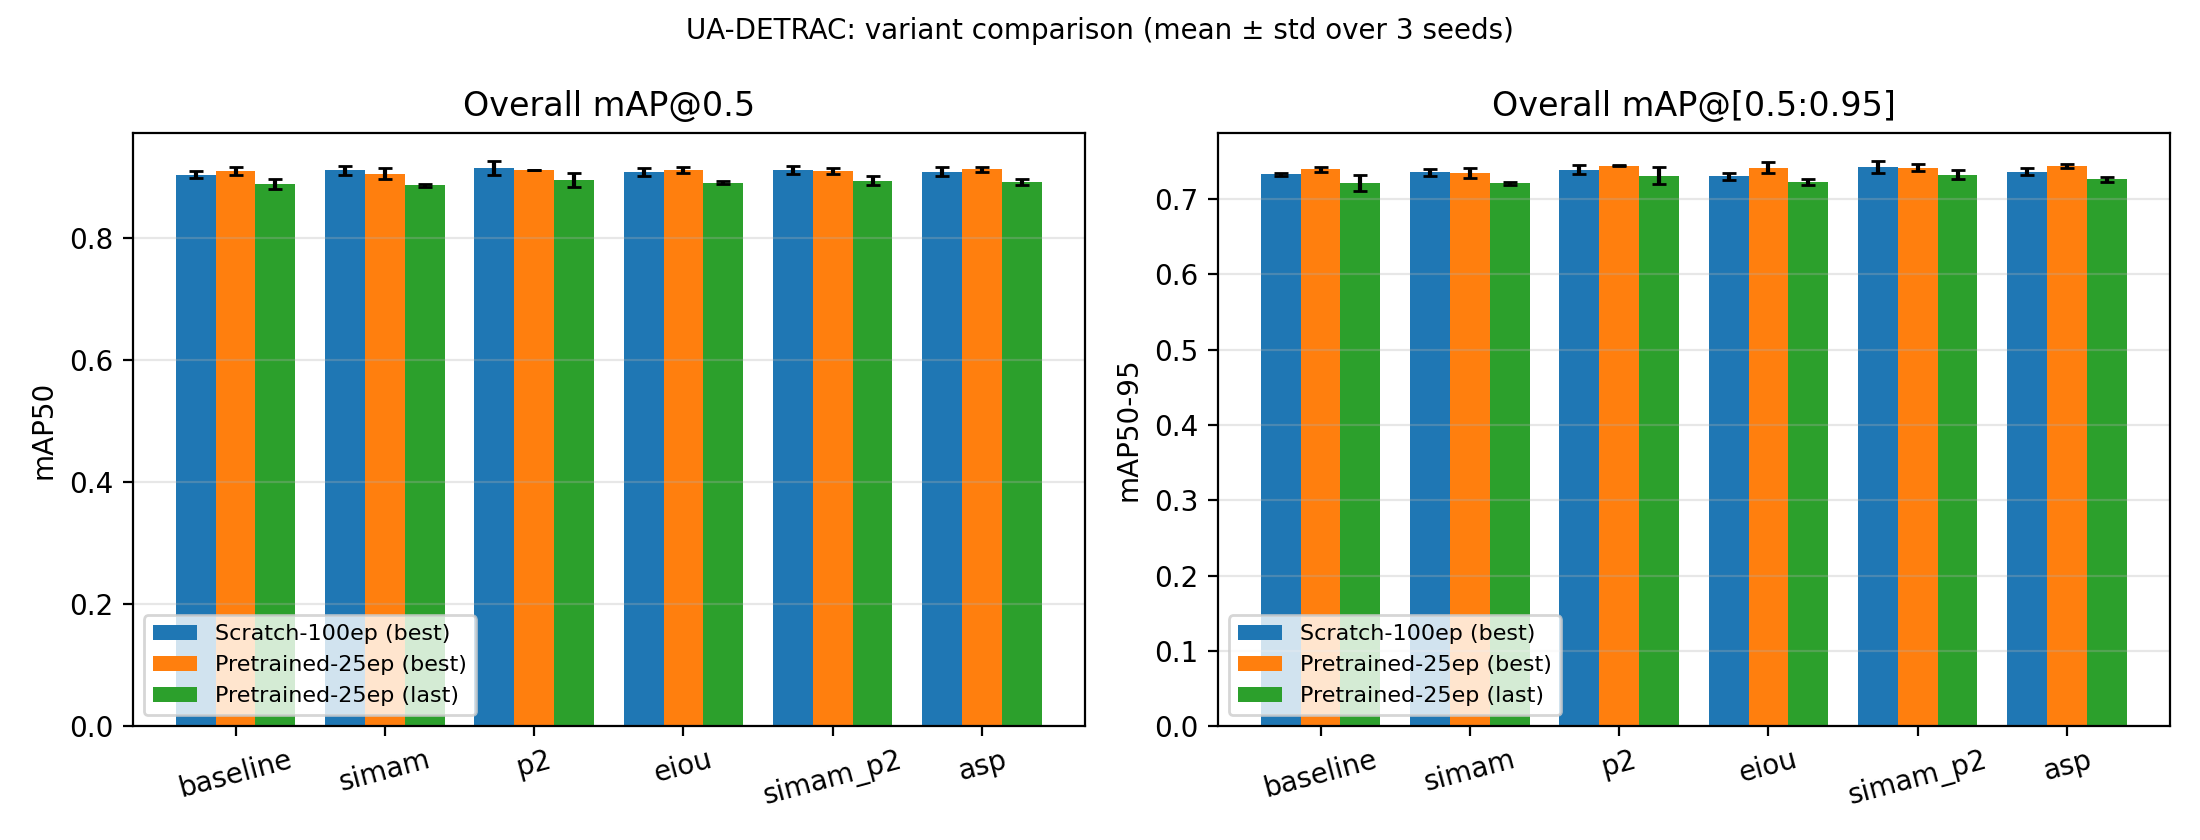
\includegraphics[width=\textwidth]{fig1_overall}
\caption{Overall mAP@0.5 (left) and mAP@[0.5:0.95] (right) for the six variants under three settings: from-scratch 100 epochs (\texttt{best}), pretrained 25 epochs (\texttt{best}) and pretrained 25 epochs (\texttt{last}). Error bars are standard deviations over three seeds. The bars are deliberately plotted from zero: the differences between variants, and between initializations, are small relative to the seed variation.}\label{fig:overall}
\end{figure*}

Figure~\ref{fig:overall} shows the same numbers graphically. Plotting from zero makes the central point of this paper visible at a glance: within a panel the six variants are visually indistinguishable relative to their error bars, whereas moving from one initialization regime to another shifts the whole group.

\subsection{Ablation analysis}

Reading Table~\ref{tab:main} as an ablation:
\begin{itemize}
\item \textbf{SimAM} changes mAP@0.5 by $+0.0012$ (\texttt{last}) and mAP@[0.5:0.95] by $-0.0005$: a null result on the overall metrics, obtained with \emph{zero} additional parameters.
\item \textbf{P2} is the only modification that leads a main column in the from-scratch regime ($0.9151$ mAP@0.5 with \texttt{best}), but it pays for it with the largest variance and the largest \texttt{best}-to-\texttt{last} drop, and it costs $51\%$ more GFLOPs.
\item \textbf{EIoU} is neutral-to-negative overall ($0.8958$ mAP@0.5 on \texttt{last}, $-0.0024$ versus baseline) and is the only variant with a significantly negative scene-level result (Section~\ref{sec:scenes}).
\item \textbf{Combining} the three modifications is not additive: SimAM+P2 is the best model under the \texttt{last} convention, but adding EIoU (ASP) removes the gain entirely and makes ASP the weakest model. Loss-level and architecture-level changes interact.
\end{itemize}

\subsection{Per-weather-scene analysis}\label{sec:scenes}

Table~\ref{tab:scenes} breaks the from-scratch results down by weather scene. Night is by far the hardest condition (baseline mAP@0.5 of $0.6335$ versus roughly $0.94$ in daylight), which is expected for a static traffic camera: headlights, low contrast and motion blur dominate.

The only statistically significant positive effects in the from-scratch regime occur in the cloudy scene, where SimAM+P2 improves mAP@0.5 by $+0.0158$ and mAP@[0.5:0.95] by $+0.0155$ ($p<0.05$), and ASP improves the same two metrics by $+0.0126$ and $+0.0133$. This is consistent with the design motivation of an energy-based attention module: under diffuse illumination the contrast between vehicle and background is reduced, and a mechanism that amplifies locally distinctive neurons has more to gain. The effect is, however, not reproduced under pretrained initialization (Section~\ref{sec:pretrained}), so we report it as a setting-dependent observation rather than as a property of the module. Figure~\ref{fig:scene} contrasts the per-scene profile of the two initialization regimes.

The only significant negative scene-level result belongs to EIoU, which reduces night-time mAP@[0.5:0.95] by $0.0133$ ($p<0.05$). Since night is the condition where localization is already hardest, this suggests that EIoU's re-weighting of the regression term interacts unfavourably with the low-contrast, high-blur regime rather than uniformly improving box regression.

\begin{table*}[t]
\caption{From-scratch per-scene results (\texttt{best} checkpoint, three seeds). Native protocol. Asterisks denote Welch $t$-tests against the baseline ($^{*}p<0.05$, $^{**}p<0.01$); all unmarked differences are non-significant.}\label{tab:scenes}%
\centering
\begin{adjustbox}{max width=\textwidth}
\begin{tabular}{@{}lcccccccc@{}}
\toprule
& \multicolumn{4}{c}{mAP@0.5} & \multicolumn{4}{c}{mAP@[0.5:0.95]}\\
\cmidrule(lr){2-5}\cmidrule(lr){6-9}
Variant & sunny & cloudy & night & rainy & sunny & cloudy & night & rainy\\
\midrule
baseline  & $0.9444$ & $0.8846$ & $0.6335$ & $0.9350$ & $0.7530$ & $0.7419$ & $0.4439$ & $0.7751$\\
simam     & $0.9484$ & $0.8901$ & $\mathbf{0.6526}$ & $0.9315$ & $0.7473$ & $0.7432$ & $0.4480$ & $0.7762$\\
p2        & $0.9438$ & $0.8984$ & $0.6396$ & $0.9370$ & $0.7466$ & $0.7524$ & $0.4457$ & $0.7803$\\
eiou      & $\mathbf{0.9530}$ & $0.8937$ & $0.6255$ & $0.9271$ & $0.7524$ & $0.7437$ & $0.4306^{*}$ & $0.7681$\\
simam\_p2 & $0.9339$ & $\mathbf{0.9004^{*}}$ & $0.6203$ & $0.9343$ & $0.7438$ & $\mathbf{0.7574^{*}}$ & $0.4453$ & $\mathbf{0.7849}$\\
asp       & $0.9409$ & $0.8972^{*}$ & $0.6205$ & $0.9354$ & $0.7478$ & $0.7552^{*}$ & $0.4438$ & $0.7758$\\
\botrule
\end{tabular}
\end{adjustbox}
\end{table*}

\subsection{Object-size analysis}\label{sec:size}

Table~\ref{tab:size} reports the COCO-protocol size breakdown. The direction of the effects is consistent with the design intent --- AP\textsubscript{medium} shows the largest positive differences ($+0.0198$ for ASP, $+0.0181$ for SimAM+P2) and AP\textsubscript{large} is essentially unchanged --- but none of the differences reaches significance.

One number deserves emphasis. The P2 variant shows a large nominal AP\textsubscript{small} gain with the \texttt{best} checkpoint ($+0.0126$), yet its three seed values are $0.4189$, $0.3642$ and $0.4205$: a standard deviation of $0.0321$, four times that of the baseline. A single-run report would thus have produced a very convincing, and very misleading, claim that the P2 head "substantially improves small-object detection". Figure~\ref{fig:size} shows the same breakdown for the pretrained regime, where the seed spread is comparable. We therefore advise against reporting size-bucketed gains without seed variation, precisely because the buckets are computed on relatively few objects and are correspondingly noisy.

\paragraph{A protocol-dependent precision effect.} The COCO evaluation that produces the size buckets also reports whole-run precision, and for SimAM in the from-scratch regime it is significantly lower than the baseline ($0.8497 \pm 0.0123$ versus $0.8817 \pm 0.0062$, a difference of $-0.0319$ with $p<0.05$), whereas the same comparison under the native protocol is not significant ($-0.0302$). This is a second instance of the sensitivity documented in Section~\ref{sec:protocols}: the scoring routine can change not only the size of a difference but whether it is significant at all. It is one reason we keep whole-run precision and recall on the native protocol and use the COCO routine only for the size buckets.

\begin{table*}[t]
\caption{COCO-protocol size breakdown (from-scratch, \texttt{best} checkpoint, three seeds). Differences versus the baseline are shown in parentheses; all are non-significant.}\label{tab:size}%
\centering
\begin{adjustbox}{max width=\textwidth}
\begin{tabular}{@{}lccc@{}}
\toprule
Variant & AP\textsubscript{small} & AP\textsubscript{medium} & AP\textsubscript{large}\\
\midrule
baseline  & $0.3886 \pm 0.0077$ & $0.6312 \pm 0.0061$ & $0.8115 \pm 0.0052$\\
simam     & $0.3983 \pm 0.0116$ $(+0.0097)$ & $0.6404 \pm 0.0283$ $(+0.0092)$ & $0.8137 \pm 0.0083$ $(+0.0022)$\\
p2        & $0.4012 \pm 0.0321$ $(+0.0126)$ & $0.6486 \pm 0.0099$ $(+0.0173)$ & $0.8100 \pm 0.0010$ $(-0.0015)$\\
eiou      & $0.4064 \pm 0.0160$ $(+0.0178)$ & $0.6421 \pm 0.0101$ $(+0.0109)$ & $0.8046 \pm 0.0090$ $(-0.0069)$\\
simam\_p2 & $0.3893 \pm 0.0213$ $(+0.0007)$ & $0.6493 \pm 0.0130$ $(+0.0181)$ & $0.8108 \pm 0.0156$ $(-0.0007)$\\
asp       & $0.3911 \pm 0.0050$ $(+0.0025)$ & $\mathbf{0.6510 \pm 0.0137}$ $(+0.0198)$ & $0.8108 \pm 0.0064$ $(-0.0007)$\\
\botrule
\end{tabular}
\end{adjustbox}
\end{table*}

\begin{figure*}[t]
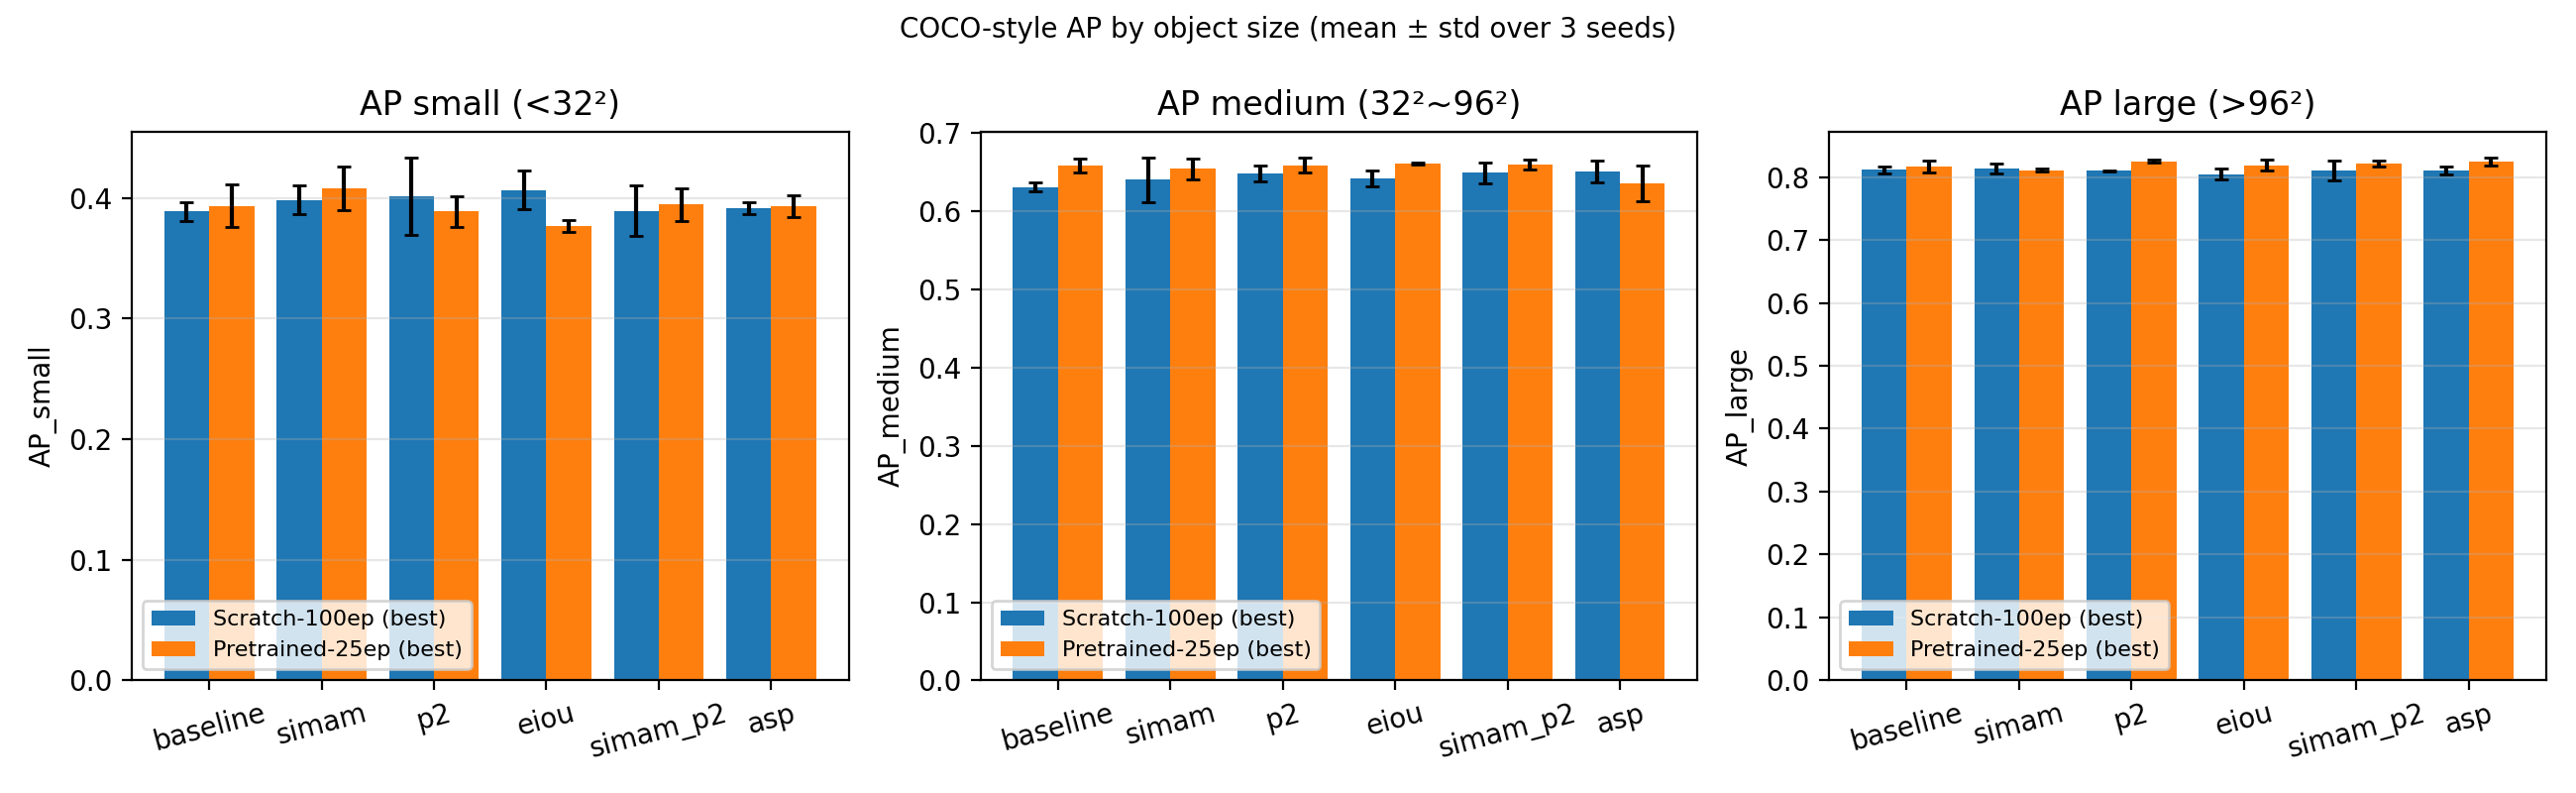
\includegraphics[width=\textwidth]{fig2_by_size}
\caption{COCO-protocol average precision by object size, from-scratch (100 epochs) versus pretrained (25 epochs), both with the \texttt{best} checkpoint. Error bars: standard deviation over three seeds.}\label{fig:size}
\end{figure*}

\subsection{Convergence and checkpoint selection}\label{sec:convergence}

Because the pretrained regime uses a fixed budget of 25 epochs, we monitored the validation metric of a 3{,}000-image stratified subset after every epoch. All six variants peak between epoch 5 and epoch 15 and then decline; four of the six variants lose between $1.2$ and $2.1$ points of mAP@0.5 from their peak to the final epoch. For two variants the ordering against the baseline even reverses between the peak and the final epoch. This is not a small fluctuation: it means that a fixed-epoch budget of 25 is already past the optimum for a COCO-pretrained model on this dataset, and that the final-epoch checkpoint is not the best available model. We therefore report both the \texttt{best} and the \texttt{last} checkpoint for the pretrained regime, and we make the selection rule explicit (Section~\ref{sec:protocols}). For the from-scratch regime, early stopping (patience 20 on the full validation set) makes the same phenomenon much less pronounced.

\subsection{Cross-initialization robustness}\label{sec:pretrained}

Table~\ref{tab:pretrained} reports the pretrained regime. Under this initialization, no variant differs significantly from the baseline on either overall metric, and the largest difference is $+0.0114$ mAP@[0.5:0.95] for SimAM+P2 with the \texttt{last} checkpoint. Within the pretrained regime, six comparisons reach significance across the two checkpoint conventions. With the \texttt{best} checkpoint, P2 improves rainy-scene mAP@[0.5:0.95] by $+0.0205$, and EIoU is significantly negative on both cloudy-scene metrics ($-0.0156$ and $-0.0161$). With the \texttt{last} checkpoint, P2 improves overall recall by $+0.0403$, SimAM improves sunny-scene mAP@0.5 by $+0.0067$, and SimAM reduces AP\textsubscript{medium} by $0.0270$.

Two comparisons between the regimes are worth stating explicitly, because they are the kind of control that is rarely reported.

\paragraph{Better initialization absorbs the gain.} Pretrained initialization raises the baseline from $0.9038$ to $0.9100$ mAP@0.5 ($+0.0062$), while the advantage of the modifications shrinks: P2 goes from $+0.0113$ to $+0.0017$ and SimAM+P2 from $+0.0078$ to $-0.0002$ relative to the baseline. In other words, a substantial part of what these lightweight modules contribute from scratch is already provided by a better starting point --- an instance of the more general observation that improvements attributed to architectural novelty often overlap with improvements obtainable from the training recipe itself \cite{he2019bag}. Reporting only the from-scratch regime --- or only the pretrained regime --- gives a misleading impression of the value of the modification.

\paragraph{The cloudy-scene effect does not replicate.} The one significant positive result of the from-scratch regime (SimAM+P2 and ASP on the cloudy scene) does not reappear under pretrained initialization, where both are non-significant and EIoU is significantly negative on the same scene. Scene-level conclusions drawn from one initialization regime should therefore be reported as regime-specific.

\begin{table*}[t]
\caption{Pretrained regime (COCO-pretrained \texttt{yolov8n.pt}, 25 epochs, no early stopping, three seeds). Native protocol, full validation set. Upper block: \texttt{best} checkpoint; lower block: \texttt{last} checkpoint. All overall differences are non-significant.}\label{tab:pretrained}%
\centering
\begin{adjustbox}{max width=\textwidth}
\begin{tabular}{@{}lccccc@{}}
\toprule
Variant & mAP@0.5 & mAP@[0.5:0.95] & AP\textsubscript{small} & AP\textsubscript{medium} & AP\textsubscript{large}\\
\midrule
\multicolumn{6}{@{}l}{\emph{\texttt{best} checkpoint}}\\
baseline  & $0.9100 \pm 0.0060$ & $0.7393 \pm 0.0036$ & $0.3933 \pm 0.0175$ & $0.6584 \pm 0.0087$ & $0.8164 \pm 0.0091$\\
simam     & $0.9057 \pm 0.0086$ & $0.7342 \pm 0.0063$ & $\mathbf{0.4078 \pm 0.0179}$ & $0.6543 \pm 0.0130$ & $0.8111 \pm 0.0018$\\
p2        & $0.9117 \pm 0.0007$ & $\mathbf{0.7442 \pm 0.0011}$ & $0.3887 \pm 0.0127$ & $0.6590 \pm 0.0097$ & $\mathbf{0.8249 \pm 0.0026}$\\
eiou      & $0.9115 \pm 0.0046$ & $0.7415 \pm 0.0077$ & $0.3766 \pm 0.0052$ & $0.6609 \pm 0.0015$ & $0.8191 \pm 0.0092$\\
simam\_p2 & $0.9097 \pm 0.0052$ & $0.7415 \pm 0.0046$ & $0.3943 \pm 0.0139$ & $0.6596 \pm 0.0065$ & $0.8213 \pm 0.0048$\\
asp       & $\mathbf{0.9126 \pm 0.0039}$ & $0.7434 \pm 0.0025$ & $0.3931 \pm 0.0088$ & $0.6357 \pm 0.0226$ & $0.8245 \pm 0.0063$\\
\midrule
\multicolumn{6}{@{}l}{\emph{\texttt{last} checkpoint}}\\
baseline  & $0.8889 \pm 0.0083$ & $0.7209 \pm 0.0103$ & $0.3806 \pm 0.0141$ & $\mathbf{0.6623 \pm 0.0077}$ & $0.8027 \pm 0.0091$\\
simam     & $0.8868 \pm 0.0026$ & $0.7206 \pm 0.0024$ & $\mathbf{0.4003 \pm 0.0173}$ & $0.6353 \pm 0.0082$ & $0.8062 \pm 0.0066$\\
p2        & $\mathbf{0.8958 \pm 0.0112}$ & $0.7307 \pm 0.0114$ & $0.3695 \pm 0.0059$ & $0.6490 \pm 0.0157$ & $0.8164 \pm 0.0043$\\
eiou      & $0.8905 \pm 0.0026$ & $0.7226 \pm 0.0045$ & $0.3745 \pm 0.0164$ & $0.6547 \pm 0.0052$ & $0.8058 \pm 0.0103$\\
simam\_p2 & $0.8940 \pm 0.0070$ & $\mathbf{0.7323 \pm 0.0055}$ & $0.3895 \pm 0.0086$ & $0.6561 \pm 0.0054$ & $\mathbf{0.8202 \pm 0.0056}$\\
asp       & $0.8916 \pm 0.0047$ & $0.7262 \pm 0.0035$ & $0.3844 \pm 0.0044$ & $0.6599 \pm 0.0158$ & $0.8077 \pm 0.0038$\\
\botrule
\end{tabular}
\end{adjustbox}
\end{table*}

\begin{figure*}[t]
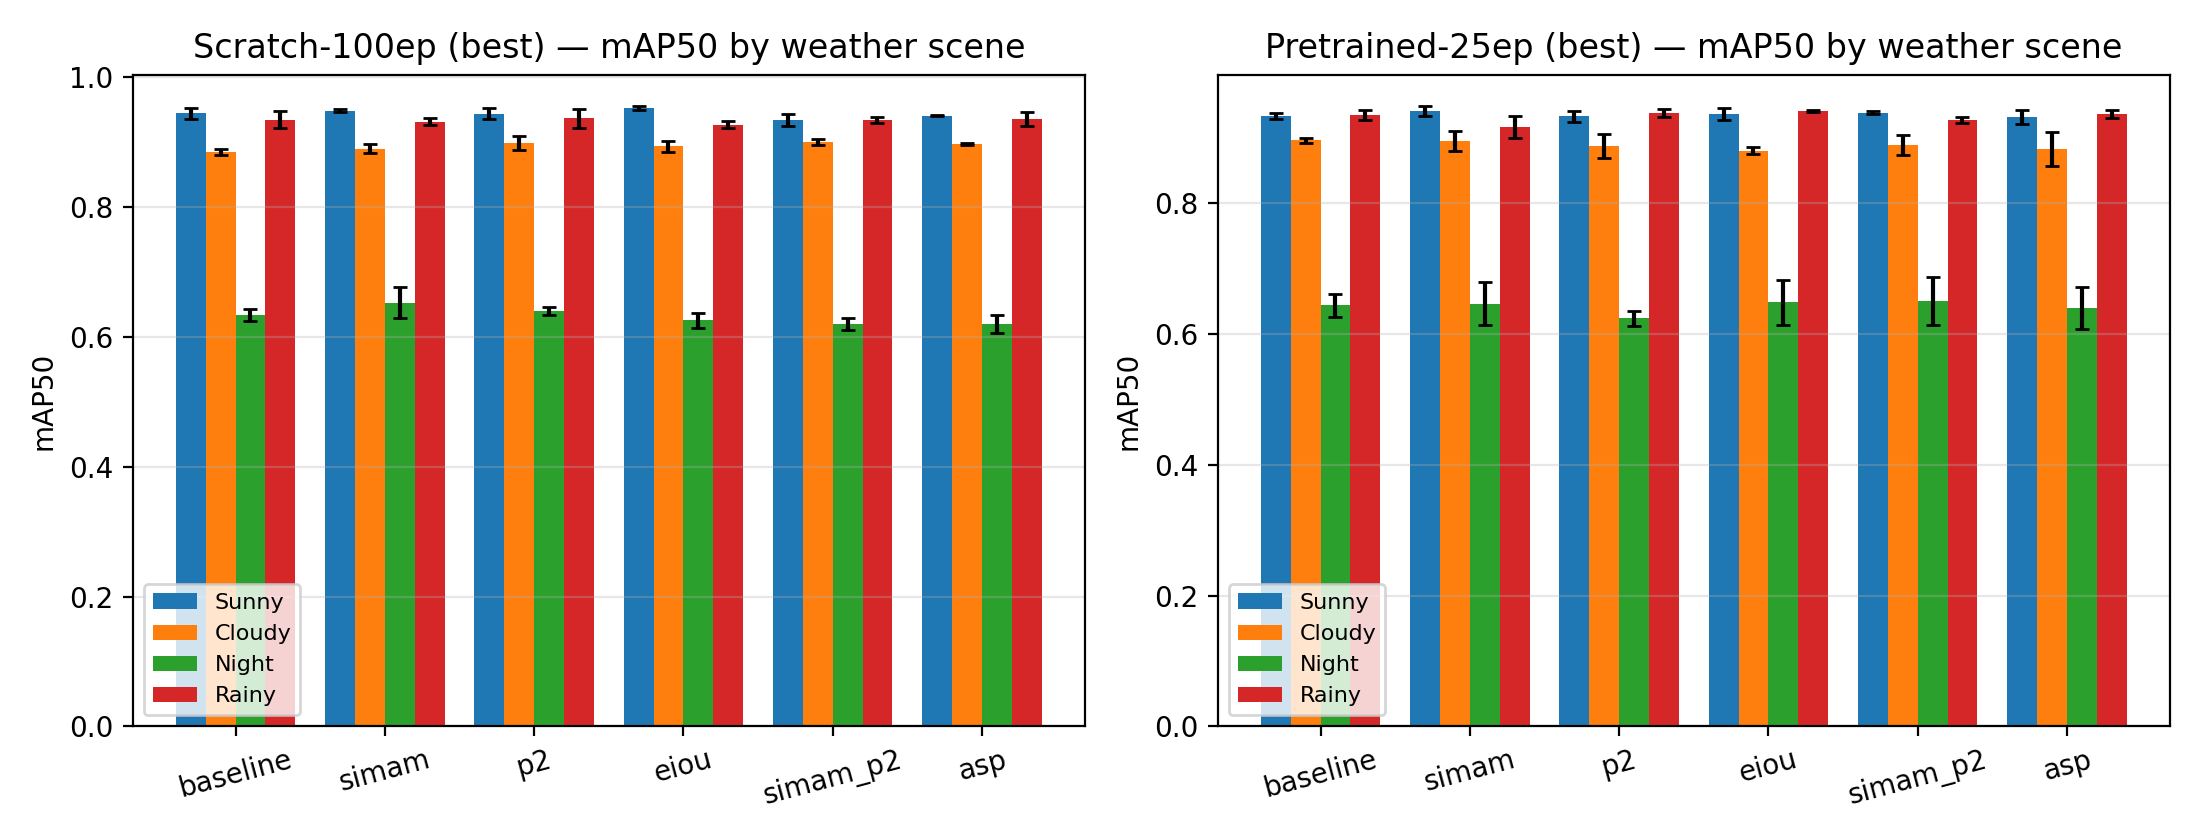
\includegraphics[width=\textwidth]{fig3_scene}
\caption{Per-scene mAP@0.5 for the six variants, from-scratch (left) and pretrained (right). Night is the dominant failure mode in both regimes.}\label{fig:scene}
\end{figure*}

\section{Discussion}\label{sec:discussion}

\subsection{What the results actually support}

Across four evaluation settings (two initializations $\times$ two checkpoint conventions) the overall differences between the six variants are small and never statistically significant. What survives this scrutiny is narrower, and we state it in the form we would defend:

\begin{enumerate}
\item \textbf{The P2 head is the most robust modification.} It leads a main column in three of the four settings (from-scratch \texttt{best} mAP@0.5; pretrained \texttt{best} mAP@[0.5:0.95], with the smallest variance of all variants; pretrained \texttt{last} mAP@0.5 and recall, the latter significant at $+0.0403$). Its cost is also the highest: $+51\%$ GFLOPs and a doubling of training memory.
\item \textbf{EIoU is not beneficial here.} It never produces a positive overall effect and is significantly negative in two scene-level comparisons. The likely reason is that EIoU re-weights the regression objective relative to the classification and assigner objectives without re-tuning the loss-balance coefficients; a fair evaluation of EIoU would re-tune the box-loss weight.
\item \textbf{SimAM is essentially free but also essentially neutral overall.} It adds zero parameters and no latency-relevant computation beyond a few element-wise operations, and it is the best variant for AP\textsubscript{small} under both pretrained checkpoints. At the same time it shows a significant AP\textsubscript{medium} loss in one setting, so the honest description is a trade-off between size regimes rather than a uniform improvement.
\item \textbf{The three modifications do not compose.} SimAM+P2 is the best variant under the from-scratch \texttt{last} convention, but adding EIoU on top removes the entire gain. Ablating modules in combination, not only individually, is therefore necessary.
\end{enumerate}

\subsection{Why small gains are expected, and why that matters}

Two mechanisms explain why the observed gains are small. The first is that the baseline is already close to the ceiling of this dataset for a nano-scale model: 100 epochs from scratch or 25 epochs of fine-tuning both reach approximately $0.90$--$0.91$ mAP@0.5, and the two initializations converge to similar accuracy. The second is that the seed-to-seed standard deviation of a nano detector on 65k images is comparable to the effect size of the modifications ($\sigma \approx 0.005$--$0.011$ versus effects of $0.001$--$0.011$). Under these conditions a single-seed comparison is not a measurement of the modification; it is largely a measurement of the seed.

This has a direct methodological consequence for the sub-field: for this class of "lightweight improvement" claims, at least three seeds, an explicitly stated checkpoint-selection rule, and a significance test should be the minimum standard. Where a full multi-seed study is impractical, reporting the \texttt{last} checkpoint (which requires no selection) removes one of the two biases at no cost.

\subsection{Practical recommendations}

\begin{itemize}
\item Report both \texttt{best} and \texttt{last} checkpoints. In our from-scratch table the difference between them is up to $2.63$ points, and the identity of the best variant changes.
\item Never mix the native and COCO scoring conventions within a table; the same checkpoint can differ by $0.9$ points.
\item Treat size-bucketed metrics as high-variance. AP\textsubscript{small} on this dataset has a standard deviation of up to $0.032$, so a gain of two points from a single run carries little information.
\item If a new module is claimed to help, verify it against a \emph{strong} baseline. A COCO-pretrained baseline absorbed $+0.0062$ mAP@0.5 of what the same modules contributed from scratch.
\item Report the cost side. Here the SimAM module is parameter-free, but the P2 level adds $51\%$ GFLOPs; a modification that improves mAP by a fraction of a point while increasing inference cost by half is a different proposition from a free one.
\end{itemize}

\subsection{Limitations}

Our study has several limitations. (i) All experiments use a single dataset and a single detector family; the conclusions concern the magnitude and reliability of the effects, not the transferability of detector architectures. (ii) With three seeds, the power of the significance tests is low: a non-significant result is inconclusive rather than evidence of no effect, and we have been careful not to present it as the latter. (iii) In the pretrained regime the fixed 25-epoch budget is past the optimum for several variants, so the reported \texttt{last} numbers understate what these models could achieve with early stopping; this is why both checkpoint conventions are given. (iv) The monitoring subset used for checkpoint selection during pretrained training is drawn from the validation split, which introduces a mild optimistic bias in the \texttt{best} rows; the \texttt{last} rows are unaffected. (v) Weather-scene labels come from the dataset's own annotation, which distinguishes only four coarse categories and does not record rain intensity or visibility, so the scene-level conclusions are sensitive to how those categories are defined.

\section{Conclusion}\label{sec:conclusion}

We presented a controlled, multi-seed, cross-initialization study of three lightweight modifications --- parameter-free SimAM attention, an additional P2 prediction level, and the EIoU regression loss --- for small-object vehicle detection on the UA-DETRAC benchmark. The headline result is deliberately unglamorous: none of the modifications improves overall mAP significantly in any of the four evaluation settings we examined, the largest difference being $+0.0114$ mAP@[0.5:0.95]. What the data do support is a narrower and more useful set of statements. The additional P2 prediction level is the most robust change, leading a main column in three of four settings and yielding a significant recall gain of $+0.0403$ under pretrained initialization, at the price of $51\%$ more GFLOPs. The EIoU loss is never beneficial on this dataset and is significantly harmful in two scene-level comparisons. The parameter-free attention module is exactly that --- free in parameters --- but its overall effect is neutral, with a small-object advantage offset by a medium-object loss in one setting. Combining all three modifications is not additive, and in one convention the full combination is the weakest model of the six.

Beyond the ablations, the study quantifies two confounds that are widespread in this literature and rarely reported: checkpoint selection, which changes the identity of the winning variant by up to $2.63$ points of mAP@0.5, and initialization strength, where a COCO-pretrained baseline absorbed $+0.0062$ mAP@0.5 and reduced a $+0.0113$ modification gain to $+0.0017$. We also document a $0.9$-point discrepancy between two scoring conventions for the same checkpoint. Our recommendation follows directly from these measurements: for claims of the "small lightweight improvement" type, report at least three seeds, state the checkpoint-selection rule, evaluate under a single consistent metric convention, and include both a from-scratch and a pretrained baseline. Doing so does not make the improvements disappear --- it makes clear which of them are real, which is the only basis on which the community can build.

\backmatter

\bmhead{Supplementary information}

The supplementary material contains: (i) the per-run metrics for all 36 training runs (18 from-scratch and 18 pretrained), including the individual seed values underlying every mean and standard deviation in this paper; (ii) the full per-scene and per-size significance tables; and (iii) the model and dataset configuration files for all six variants. The training and evaluation scripts and the command lines that reproduce every run are openly available in the repository given under Code availability.

\bmhead{Acknowledgements}

The authors thank the maintainers of the UA-DETRAC benchmark and of the Ultralytics library. Computational resources were provided by a rented NVIDIA RTX 4090 D instance and by a local NVIDIA RTX 4060 Laptop GPU.

\section*{Declarations}

\begin{itemize}
\item \textbf{Funding:} Not applicable. This research received no external funding.
\item \textbf{Conflict of interest/Competing interests:} The authors declare no competing interests.
\item \textbf{Ethics approval and consent to participate:} Not applicable. This study uses only a publicly available, fully anonymized vehicle-detection dataset and involves no human or animal subjects.
\item \textbf{Consent for publication:} Not applicable.
\item \textbf{Data availability:} The UA-DETRAC dataset is publicly available from its official benchmark website. The derived evaluation tables, per-run metrics and figure-generating scripts that support the findings of this study are included as supplementary material and are also available from the corresponding author on reasonable request.
\item \textbf{Materials availability:} Not applicable.
\item \textbf{Code availability:} The complete source code, model configurations, training and evaluation scripts, significance-testing utilities and the scripts that regenerate every table and figure in this paper are openly available at \url{https://github.com/kzzzt/UA-DETRAC-YOLOv8n-ASP}.
\item \textbf{Author contribution:} Z.K. designed the study, implemented the model variants and the analysis pipeline, conducted all experiments and analyses, and wrote the manuscript. X.L. supervised the study and revised the manuscript. Both authors read and approved the final manuscript.
\end{itemize}

\begin{appendices}

\section{Reproducibility details}\label{app:repro}

\paragraph{Data preparation.} UA-DETRAC annotations are converted from the official XML files to YOLO format with a sequence-disjoint split; images are not resized before training, and letterboxing is applied by the training pipeline. Weather labels are read from the official \texttt{sence\_weather} field; when absent, they are estimated from image luminance statistics. Frame indices in the XML annotations are 1-based, a detail that silently shifts every label by one frame if ignored.

\paragraph{Effective batch size.} Ultralytics scales the optimizer step by a nominal batch size (\texttt{nbs}=64), accumulating gradients whenever the per-step batch is smaller. For batch sizes 16 and 32 the accumulation factors are 4 and 2, so the number of optimizer steps per epoch, the learning-rate schedule and the weight-decay scaling are identical. This is what makes the batch-16 P2 variants comparable with the batch-32 baseline; the only remaining difference is the BatchNorm batch statistics.

\paragraph{Environment-induced fallbacks.} Two adaptive fallbacks of the training framework were observed during the server experiments and are documented here for transparency. (i) On CUDA out-of-memory, the framework halves the per-step batch and retries; this occurred once, for a single variant in one seed, whose effective batch therefore remained 64 (accumulation 4 instead of 2) but whose BatchNorm statistics differ. (ii) The task-aligned assigner has an independent out-of-memory fallback that affects only the assignment computation of the affected iteration and does not change the batch size. Across 18 training runs and approximately 450 epochs, three such events occurred in total, each affecting at most one epoch. We list them because they are invisible in the final checkpoints but relevant to exact reproduction.

\paragraph{Evaluation commands.} Overall and per-scene metrics are produced by evaluating each checkpoint on the full validation set under the native protocol; size-bucketed metrics are produced by a separate COCO-protocol evaluation of the same checkpoints. Both routines iterate over exactly the same 16{,}645 validation images, and the reported \texttt{all} column of the size table is cross-checked against the native protocol to detect configuration mistakes.

\section{Per-run results}\label{app:runs}

Table~\ref{tab:perrun} lists the individual runs that underlie the means in Table~\ref{tab:pretrained}; the from-scratch runs are listed in the supplementary material. Reporting individual runs is what allows the reader to recompute the significance tests, and it also exposes occasional outliers (for example, an early peak followed by a long decline) that a mean would hide.

%% Deliberately not a float. As the last object of the appendices, this table was
%% deferred by LaTeX twice: first as a table*, which printed it inside the
%% reference list, and then as a non-starred table with [htbp], which still put it
%% on the first bibliography page and left the preceding page almost empty.
%% Defining \@captype makes \caption emit the class's normal table caption without
%% a float, so the table is typeset exactly where it is written. This is the same
%% mechanism the caption package uses for \captionof. \makeatletter is required:
%% outside it, @ is not a letter and \def\@captype would define \@ instead, which
%% is what made \caption report "Caption outside float".
\begin{center}
\makeatletter\def\@captype{table}\makeatother
\caption{Pretrained regime, individual runs (\texttt{best} checkpoint, native protocol, full validation set).}\label{tab:perrun}%
\tablebodyfont
\begin{tabular*}{\textwidth}{@{\extracolsep\fill}lcccccc}
\toprule
Run & mAP@0.5 & mAP@[.5:.95] & Run & mAP@0.5 & mAP@[.5:.95]\\
\midrule
baseline\_s0 & $0.9034$ & $0.7352$ & simam\_p2\_s0 & $0.9151$ & $0.7465$\\
baseline\_s1 & $0.9151$ & $0.7421$ & simam\_p2\_s1 & $0.9094$ & $0.7406$\\
baseline\_s2 & $0.9114$ & $0.7405$ & simam\_p2\_s2 & $0.9047$ & $0.7375$\\
simam\_s0 & $0.9134$ & $0.7394$ & asp\_s0 & $0.9093$ & $0.7426$\\
simam\_s1 & $0.8964$ & $0.7272$ & asp\_s1 & $0.9169$ & $0.7462$\\
simam\_s2 & $0.9073$ & $0.7360$ & asp\_s2 & $0.9116$ & $0.7415$\\
p2\_s0 & $0.9110$ & $0.7441$ & eiou\_s0 & $0.9062$ & $0.7390$\\
p2\_s1 & $0.9123$ & $0.7454$ & eiou\_s1 & $0.9137$ & $0.7501$\\
p2\_s2 & $0.9118$ & $0.7432$ & eiou\_s2 & $0.9146$ & $0.7354$\\
\botrule
\end{tabular*}
\end{center}

\end{appendices}

\bibliography{refs}% common bib file

\end{document}
